% 5章
\chapter{数値実験}

研究で新たに実装した歩行者工一ジェントおよび介護シミュレーションの定量的な評価性能を検証するために,シミュレーション実験を行った.
この章では,実験で用いた環境設定と,実験結果をどのような評価指標で判断したか,またその結果と考察についてまとめている.

\section{実験条件}

今回の実験では介護環境として,図\ref{environment}に示すように,15m四方の二次元平面と,排泄場所としてのトイレをその上部に設置した.

\begin{figure}[htb]
\begin{center}
 
\includegraphics[scale=0.5]{figures/environment.png}
 \caption[実験環境]{実験環境 \label{environment}}
\end{center}
\end{figure}

この環境の中で,介護者と被介護者の可視化をおこなっていく.今回の実験では,介護における技術を導入した際に,それが介護環境にどのようなインパクトをあたえるのかについて検証を行うことが目的なので,介護者の数は1人,被介護者の数は16人と設定し,比較的大きい施設を対象とした.第4章で述べた適切なタイミングで介護要望フラグをたてる被介護者,早いタイミングで介護要望フラグをたてる被介護者の被介護者,遅いタイミングで介護要望フラグをたてる被介護者の被介護者の3種類のエージェントが,介護施設内の自由時間である2時間の間にいかなる回数にわたって排泄介助を行うことが必要か,またその介助は本当に必要であったのかということを確かめる実験をおこなう.3種類の被介護エージェントを\ref{experiment}のように組み合わせた6パターンにおいて,相互作用を確認し,それを本章で示す評価指標で評価する.

\begin{figure}[htb]
\begin{center}
 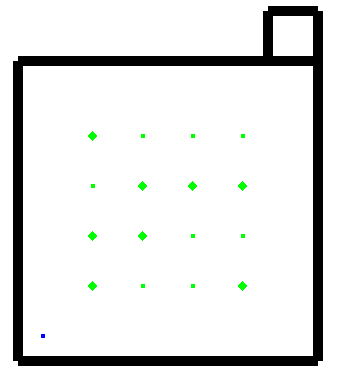
\includegraphics[scale=0.5]{figures/health_urinate.png}
 \caption[適切なタイミングで介護要望フラグをたてる被介護者と遅いタイミングで介護要望フラグをたてる被介護者の場合の可視化]{適切なタイミングで介護要望フラグをたてる被介護者と遅いタイミングで介護要望フラグをたてる被介護者の場合の可視化 \label{health_urinate}}
\end{center}
\end{figure}

\begin{figure}[htb]
\begin{center}
 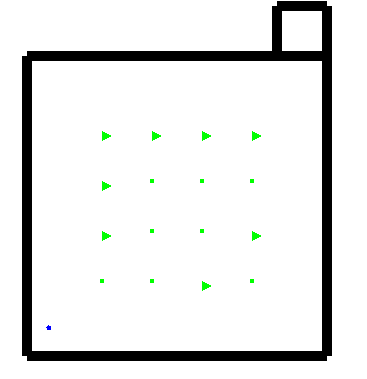
\includegraphics[scale=0.5]{figures/health_frequently_urinate_v1.png}
 \caption[適切なタイミングで介護要望フラグをたてる被介護者と早いタイミングで介護要望フラグをたてる被介護者の場合の可視化]{適切なタイミングで介護要望フラグをたてる被介護者と早いタイミングで介護要望フラグをたてる被介護者の場合の可視化 \label{health_frequently_urinate_v1}}
\end{center}
\end{figure}

\begin{figure}[htb]
\begin{center}
 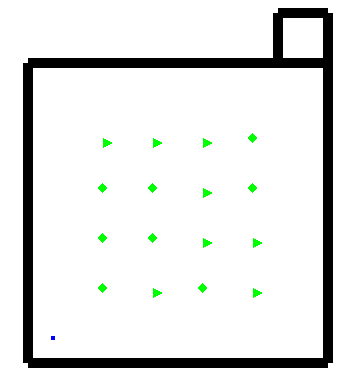
\includegraphics[scale=0.5]{figures/dementia_urinate_v1.png}
 \caption[遅いタイミングで介護要望フラグをたてる被介護者と早いタイミングで介護要望フラグをたてる被介護者の場合の可視化]{遅いタイミングで介護要望フラグをたてる被介護者と早いタイミングで介護要望フラグをたてる被介護者の場合の可視化 \label{dementia_urinate_v1}}
\end{center}
\end{figure}

\begin{table}[htb]
  \caption[実験条件]{実験条件}
  \label{experiment}
  \centering
  \begin{tabular}{r|c|c|c|c|c|c|c}
     & Case1 & Case2 & Case3 & Case4 & Case5 & Case6 & Case7 \\ \hline
    適切 & 100% & 0% & 0% & 50% & 50% & 0% & 33% \\
    早い & 0% & 100% & 0% & 50% & 0% & 50% & 33% \\
    遅い & 0% & 0% & 100% & 0% & 50% & 50% & 33% \\
    \end{tabular}
\end{table}

表\ref{experiment}に示したように,Case1は、健常の被介護者(技術の補助を受けた被介護者)が100%の状態,Case2は早いタイミングで介護要望フラグをたてる被介護者の被介護者が100%の状態,Case3は遅いタイミングで介護要望フラグをたてる被介護者の被介護者が100%の状態,Case4は、健常の被介護者(技術の補助を受けた被介護者)と早いタイミングで介護要望フラグをたてる被介護者の被介護者が50%ずつの状態,Case5は健常の被介護者(技術の補助を受けた被介護者)と遅いタイミングで介護要望フラグをたてる被介護者の被介護者が50%ずつの状態,Case6は早いタイミングで介護要望フラグをたてる被介護者の被介護者と遅いタイミングで介護要望フラグをたてる被介護者の被介護者が50%ずつの状態である.なお,Case7に関しては,16人という設定上同じ設定で3等分できなかったので,(5,5,6),(5,6,5),(6,5,5)の3回の平均値をとることにした.なお,Case1は,適切なタイミングで介護要望フラグを立てる設定であり,被介護者に適切なサポートが入っている状態であるので,実験結果はCase1とそれぞれを比較することで技術によるサポートのインパクトを評価することができる.

\section{介護挙動の基本的な検証}

本シミュレータが現実を反映できているのかについて,簡単な検証を行った.介護アラートを出す条件を,適切なタイミングで介護要望フラグをたてる被介護者の場合は100ml以上になった時点,早いタイミングで介護要望フラグをたてる被介護者の場合は75ml以上になった時点,遅いタイミングで介護要望フラグをたてる被介護者の場合は150ml以上で介護アラートを発する設定にし,2時間シミュレータを回した.その結果,適切なタイミングで介護要望フラグをたてる被介護者の場合は,2時間に1回トイレに行くという結果を得ることができた.これは実際のデータと比較しても整合性のある値となった.この結果を表\ref{number_of_urination}に示す.なお,実験では16人の被介護者が存在するので実際は数値を16で割った数字が一人当たりの回数となっている.

\begin{table}[htb]
  \caption[被介護者ごとの排尿回数]{被介護者ごとの排尿回数}
  \label{number_of_urination}
  \centering
  \begin{tabular}{r|c|c|c}
     & 適切なタイミング & 早いタイミング & 遅いタイミング \\ \hline
    一回目 & 15 & 21 & 6 \\
    二回目 & 15 & 22 & 5 \\
    三回目 & 16 & 26 & 5 \\
  \end{tabular}
\end{table}

\section{評価指標}

本研究の目的は,疾患のある被介護者,すなわち現状介護者の負担増の原因となっており,被介護者自身も自らの排泄が負担となっているようなケースにおいて,技術の導入を行うことでどれだけの効果が得られるのかを可視化するというものである.そこで,評価指標として,介護者の負担を示す指標として,行った介護回数,被介護者が強いられた負担を示す指標として,排泄に行くべきである尿量の状態,あるいは自身が排泄に行きたいと感じている状態から実際に排泄を行うまでの時間を計測し,それを総我慢時間とする.

\section{結果および考察}

図\ref{result_v1}に,介護者・被介護者の割合をCase1からCase7までそれぞれ変化させた場合のシミュレーション結果(10回の試行の平均値)を示す.表\ref{relative_error}に,それぞれの具体的な数値とCase1に対する相対誤差を示した.次に表\ref{number_of_care}に,Caseごとの介護回数とCase1に対する相対誤差を示した.

\begin{figure}[htb]
\begin{center}
 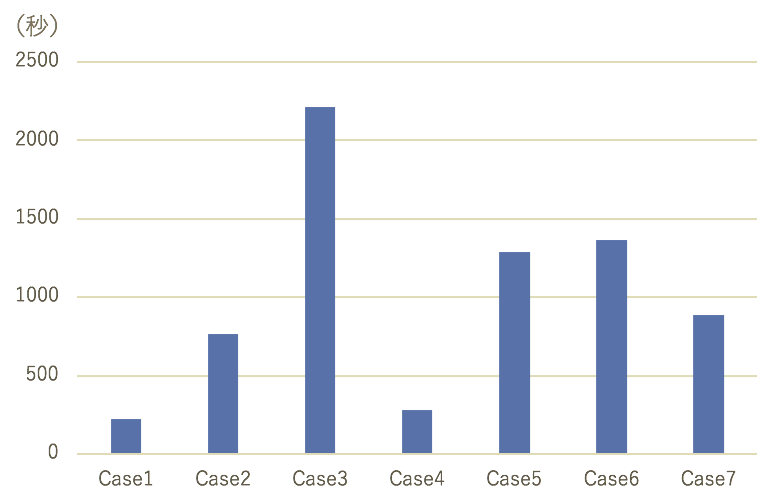
\includegraphics[scale=0.5]{figures/result_v1}
 \caption[実験結果]{実験結果 \label{result_v1}}
\end{center}
\end{figure}

\begin{table}[htb]
  \caption[Caseごとの我慢時間]{Caseごとの我慢時間}
  \label{relative_error}
  \centering
  \begin{tabular}{r|c|c|c|c|c|c|c}
     & Case1 & Case2 & Case3 & Case4 & Case5 & Case6 & Case7 \\ \hline
    我慢時間 & 220.1 & 764.0 & 2213.5 & 278.4 & 1285.9 & 1363.7 & 884.3 \\
    相対誤差 & & 2.47 & 9.05 & 0.26 & 4.84 & 5.19 & 3.02 \\
    \end{tabular}
\end{table}


\begin{table}[htb]
  \caption[Caseごとの介護回数]{Caseごとの介護回数}
  \label{number_of_care}
  \centering
  \begin{tabular}{r|c|c|c|c|c|c|c}
     & case1 & Case2 & Case3 & Case4 & Case5 & Case6 & Case7\\ \hline
    介護回数 & 15-16 & 21-26 & 5-6 & 19-21 & 9-10 & 16-17 & 15-18\\
    相対誤差 & & 0.50 & -0.65 & 0.31 & -0.37 & 0.07 & 0.09 \\
    \end{tabular}
\end{table}

Case2については,過剰介護が問題であると考えられる.適切なタイミングで介護要望フラグをたてる被介護者の場合と比べ,50%以上も介護士の労働力に悪影響を与えているといえる.早いタイミングで介護要望フラグをたてる被介護者の場合は,単純にトイレに行かないという選択肢を現場で取ることができないので,おむつなどで現場では対応していると考えられる.しかしおむつは,被介護者の自立意識を妨げるツールであるので,その使用については注意が必要である.どのタイミングでおむつをつけることを決め,どの時点でつけることをやめるのか,その意思決定基準はブラックボックスになっている.しかしCase4の結果を見ると,被介護者の我慢時間がCase1との相対誤差が小さいことに加えて,実際の介護回数も相対誤差0.31に留まっている.すなわちシミュレーションによって,高齢者施設がどういった状態の被介護者を受け入れるか,あるいはどの被介護者同士を同じ部屋に入れ,一人の被介護者に対応させるのかといった人事配置について示唆を得ることができることを示している.

Case3の総我慢時間が,もっとも高いものとなっているが,これは被介護者が本来なら排泄に向かうべき尿量であるのにも関わらず,無意識のうちに我慢をしてしまい,介護者にアラートを出した時点ですでにかなりの時間を待ち時間として計測してしまっていることが原因であることが考えられる.逆に言えば,技術を導入することでCase1の状態へと環境を変えることで,被介護者の我慢時間を述べ約2000秒も短縮することができる.

Case5では,数値上は相対誤差がかなり少ないように見えるが,実際は適切なタイミングで介護要望フラグをたてる被介護者と遅いタイミングで介護要望フラグをたてる被介護者の被介護者の間の待ち時間の差が大きく,適切なタイミングで介護要望フラグをたてる被介護者の割合が減ったことで,適切なタイミングで介護要望フラグをたてる被介護者がアラートを出した際にすぐ介護してもらえたということがあげられる.実際の現場では,被介護者の要介護によって,どの介護者がつくべきかということが事前情報として与えられているため,このような複雑な状況にも対応していけるような環境をつくっているという示唆を得ることができる.今後の検討課題として,そういった事前情報の有無によって,どの介護者と被介護者をマッチングさせるのかということが挙げられる.具体的にどのような事前情報に基づいて意思決定が行われているのか今後の調査課題である.

Case6は我慢時間こそ多いものの,介護回数についてはCase1とそれほど違いが出ていない.しかし,これも早いタイミングで介護要望フラグをたてる被介護者の被介護者に対する介護が多く,遅いタイミングで介護要望フラグをたてる被介護者の被介護者に対する介護回数が少ないので,合計回数が相殺してCase1と近い値が出てしまったためである.

Case7について,介護回数では早いタイミングと遅いタイミングの被介護者同士が打ち消しあうので,Case1と差が出ないことは直感的に正しい.我慢時間をCase6と比較した際にも,約2/3倍であり適切なタイミングではない被介護者の数におおむね比例している.
